Intuitively speaking, the communication time should increase when more peers join a training setup, as more data needs to be sent between each peer.
However, looking more closely at the time of the hybrid-cloud experiments in the ~\Cref{fig:cv-private-hybrid-cloud-granularity,fig:nlp-private-hybrid-cloud-granularity,fig:cv-research-hybrid-cloud-granularity}, the communication time seems to decrease while the number of GPUs increases.

\textbf{Communication time can decrease with more peers.} The intercontinental experiments in ~\Cref{sec:geodistributed-performance} showed that we pay a one-time penalty for the slowest interconnect.
However, for those experiments, the GPU groups on each continent had relatively poor connectivity with each other but were very well connected within their group.
For the hybrid-cloud experiments, the on-premise network connectivity poses a bottleneck for communication.
Let us compare the granularity of the experiments for E-B (\Cref{fig:cv-private-hybrid-cloud-granularity}), which uses T4 GPUs in the US as an additional cloud resource.
\textit{Both} the computation and communication time decrease with the number of GPUs, even increasing the granularity from 1.98 at E-B-2 to 2.15 at E-B-4.
This is surprising since, usually, with more peers, the communication time should increase, and the US-EU communication bottleneck should slow us down to the same extent as the E-B-1 experiment.
This reduction is a Hivemind-specific anomaly, as it uses a single TCP stream per peer.
With TCP, there needs to be an acknowledgment (ACK) of each packet by the receiving peer, which is impacted by the connection's latency.
In our high latency network between continents, the round trip time (RTT) of 300-318ms limits the maximum bandwidth a single TCP stream to 50-80~Mbits.
\begin{figure}
    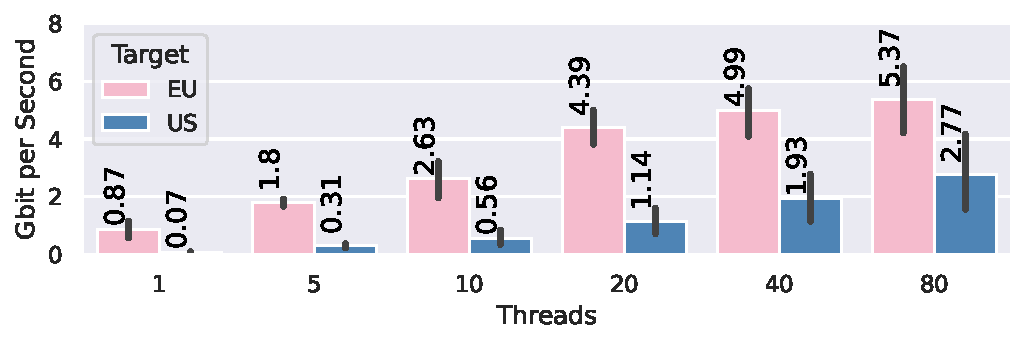
\includegraphics[width=0.45\textwidth]{figures/misc/multi-threaded-iperf-eu-us}
    \vspace{-15pt}
    \caption{Multithreaded iperf throughput in Gbits from the EU RTX8000 to GC-US/EU.}
    \label{fig:multi-threaded-iperf-eu-us}
    \vspace*{-6mm}
\end{figure} 
However, a way to improve link utilization is to use multiple streams, one for each peer, which we encounter in experiments E-(B|C)-2,4,8.
The US VMs communicate in parallel with the RTX8000, which receives at a rate of up to 670~Mbits and transmits at a rate of up to 600~Mbits in the communication rounds.
Due to the parallel streams, we achieve a communication time reduction with an increased amount of peers.
To verify the potential gains, we perform a microbenchmark of the multi-stream bandwidth from the RTX8000 to the EU and US data centers (\Cref{fig:multi-threaded-iperf-eu-us})\footnote{Note that the single-threaded throughput is slightly faster than our original measurements, due to measuring at a different time of day.}.
Although there is wide variation, likely due to network utilization, with 80 clients, we achieve a maximum bandwidth of 6 Gbits within the EU and up to 4 Gbits to the US. 
While larger peer groups and, consequently, larger models benefit from multi-peer communication by default and do not see significant changes in communication time, small models in unevenly distributed VMs setups can be disproportionately affected.
The same trend can be observed in all high latency experiments (i.e., between the EU and the US), e.g., E-B, E-C for CV and NLP, and F-B and F-C for CV.
In summary, uneven distribution of computational resources in high-latency networks (e.g., intercontinental) can reduce communication time with Hivemind due to more parallelism, lessening the impact of low bandwidth for a single data stream.

\textbf{Cost analysis.} The DGX-2 (8xV100) node from ~\Cref{sec:hybrid-cloud-performance} represents server-grade hardware that could be used to train models.
However, how does it compare in throughput per \$ to all of our distributed cloud experiments?
\begin{figure}
    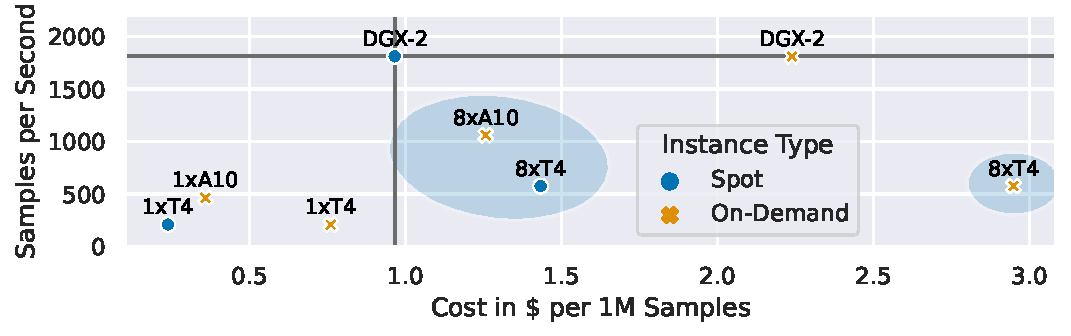
\includegraphics[width=0.49\textwidth]{figures/misc/nlp_cost_per_sps_comparison}
    \vspace{-25pt}
    \caption{Tradeoff between cost per sample (x-axis) and model throughput (y-axis) for RoBERTaXLM at different instance types. Our training setups (circled), that are due the low granularity of the NLP model, neither cheaper, nor faster than the centralized offering (DGX-2).} 
    \label{fig:nlp-sps-trade-off}
    \vspace*{-4mm}
\end{figure}
The ~\Cref{fig:cv-sps-trade-off} (CV) and ~\Cref{fig:nlp-sps-trade-off} (NLP) show the complete cost analysis of the DGX-2, the 8xT4 experiments, and the 8xA10 experiments for spot and on-demand pricing. We use the internal egress costs from ~\Cref{fig:multi-cloud-costs-d3} as a reference for the 8xT4 setup.
For simplicity, we compare the spot pricing without interruptions, as we assume that a new VM can be spun up fast enough not to affect the training throughput in the long run.
We mark the centralized baseline (DGX-2) cost per 1M samples and the throughput in samples per second with a horizontal and vertical line.
This means that we are cheaper to the left to the vertical line, and above the horizontal line, we are faster (and vice versa).
We circle the new value propositions that we enable in both figures.

A spot DGX-2 costs at the time of writing 6.30\$/h (14.60\$/h on-demand) in GC US, which makes it the best value proposition for the low granularity NLP task.
It is followed by the 8xA10, which are 41\% slower and 30\% more expensive than the DGX-2 (\Cref{fig:nlp-sps-trade-off}). 
The 8xT4 experiments are even more expensive, as the internal egress costs take up more than half of the costs, making them the worst-value proposition.
However, for CV, we manage to provide two new offerings: First, the 8xA10, which is both 50\% faster and 49\% cheaper than the DGX-2, and 8xT4, which is 58\% cheaper than DGX-2, while being 37\% slower (\Cref{fig:cv-sps-trade-off}).
The CV model can be scaled more easily due to its initially high granularity, which makes the very competitive offering of 0.6\$/h per A10 from LambdaLabs an excellent value proposition.
However, while we only evaluated eight T4 GPUs for our GC-based experiments, with a granularity of 5.19 (CV A-8 in ~\Cref{fig:geo-dist-us-only-granularity}), there is ample space to scale even further.
It is important to note that LambdaLabs does not charge for any data egress, but GC does with 0.01\$/GB, and the 8xT4 experiment is still cheaper.  
While LambdaLabs is often at capacity, Google Cloud positions itself as a hyperscaler with the advantage of rarely being at max occupancy. 

In summary, the lower spot prices for older GPUs allow us to train models more cost-efficiently when task granularity allows it and get more value per \$ when training on the 8xT4 or 8xA10 compared to an DGX-2 node.
Distributed spot instance pricing opens up a new value proposition compared to on-demand offerings that can even compete with the competitive pricing of smaller cloud providers.